\documentclass[10pt,a4paper]{article}
\usepackage[utf8]{inputenc}
\usepackage[italian]{babel}
\usepackage{amsmath}
\usepackage{cancel}
\usepackage{amsmath}
\usepackage{ amssymb }
\usepackage{placeins}
\usepackage{url}
\usepackage{soul}
\usepackage{amsfonts}
\usepackage{booktabs}
\usepackage{braket}
\usepackage{amssymb}
\usepackage{graphicx}
\usepackage{caption}
\usepackage{subcaption}
\usepackage{siunitx}
\usepackage{diagbox}
\usepackage{slashbox}
\usepackage{comment}
\usepackage{wrapfig}
\usepackage[dvipsnames]{xcolor}
\usepackage[left=2cm,right=2cm,top=2cm,bottom=2cm]{geometry}
\newcommand{\rem}[1]{[\emph{#1}]}
\newcommand{\exn}{\phantom{xxx}}
\definecolor{LightGray}{gray}{0.95}
\usepackage[colorlinks = true,
            linkcolor = black,
            urlcolor  = blue,]{hyperref}
\usepackage{minted}
\usepackage[version=4]{mhchem}

\author{Lorenzo Zaffina}
\title{Impiego di transmoni superconduttori\\ per la rivelazione di Assioni e materia oscura
}
\begin{document}
\date{\today}
\maketitle

Questi sono degli appunti personali, da usare come scaletta per la presentazione della tesi triennale. Li ho scritti un po' di fretta quindi è possibile che siano presenti errori.


\section{Gli assioni}

Uno dei problemi aperti della fisica moderna è quello riguardante la \textbf{materia oscura}. A supporto della sua esistenza vi sono innumerevoli osservazioni astronomiche, ma la sua natura fondamentale rimane ignota. In particolare, si stima che solo il 15\% della materia dell’universo sia costituita da particelle del Modello Standard, mentre il restante \textbf{85\%} è imputabile alla materia oscura.\\

L’idea degli assioni venne proposta per la prima volta nel 1977 da Peccei e Quinn per risolvere il problema della \textbf{mancata osservazione della violazione di CP nell’interazione forte tra quark}. Queste ipotetiche particelle (insieme alle cosiddette ALPs, Axion-Like Particles), dovrebbero interagire estremamente poco con le particelle del modello standard, e perciò rappresentano alcuni tra i più validi candidati per la materia oscura. \\

Per la rivelazione di assioni si sfrutta l’accoppiamento del campo assionico (A) con il campo elettromagnetico. In particolare, la costante di accoppiamento $g_{\alpha\gamma\gamma}$ è proporzionale alla massa a riposo dell’assione $m_ac^2$.  Questo vincolo fornisce un’indicazione che guida la ricerca sperimentale, tuttavia si effettuano esperimenti volti a sondare tutto il piano dei parametri ($g_{\alpha\gamma\gamma}$ - $m_ac^2$)  alla ricerca delle più generali ALPs.

\section{Techniche di rivelazione}

La ricerca sperimentale degli assioni viene condotta essenzialmente su due fronti: il primo è la ricerca di assioni prodotti da fonti astronomiche, il secondo consiste in esperimenti condotti in laboratorio basati sulla generazione e rigenerazione di fotoni.\\

Nel primo caso l’idea è quella di rivelare i fotoni prodotti dalla riconversione degli assioni di origine cosmica. In particolare, si lavora ai cosiddetti \textbf{Elioscopi}, il cui scopo è quello di rivelare assioni prodotti nel nucleo solare, che vengono riconvertiti in fotoni in potenti magneti puntati verso il sole. Un esempio di Elioscopio è il CAST - CERN Axion Solar Telescope, che ha preso dati dal 2013 e 2016, contribuendo a definire i vincoli sperimentali alla massa degli assioni e al loro accoppiamento con i fotoni.\\

Un altro tipo di esperimenti che guardano ad assioni cosmici sono gli \textbf{aloscopi}, il cui obiettivo è rivelare assioni provenienti dall’alone galattico mediante il loro accoppiamento con i fotoni. \\
\textit{Haloscopes such as  MADMAX look for axions that would be the dominant constituents of the dark matter halo of our galaxy by using microwave resonators immersed in a magnetic field.}\\

I principali esperimenti in laboratorio sono i cosiddetti “\textbf{Light shining through a wall}” (LSW), in cui dei fotoni, sottoposti ad un intenso campo magnetico che ne permette la conversione in assioni (o ALPs), vengono inviati verso una barriera ottica. Dall’altro lato della barriera è presente un campo magnetico che permette la riconversione degli eventuali assioni che hanno superato la barriera in fotoni, i quali verranno rivelati.\\



In tutti questi casi, la rivelazione di assioni, o di ALPs in generale, si basa sull’\textbf{accoppiamento con i fotoni}. Siccome tali particelle sono estremamente poco interagenti, la sfida sperimentale è quella di riuscire a rivelare \textbf{singoli fotoni}, tipicamente nelle microonde.
L’idea è quella di usare a tale scopo dei Qubit superconduttori chiamati trasmoni.


\section{I Qubit}

\textbf{Nota:} Per questa parte ho seguito estensivamente il talk diponibile al seguente link \url{https://www.youtube.com/watch?v=t5nxusm_Umk}.
\subsection{Atomi e sistemi a due livelli}
Un qubit è sostanzialmente un \textbf{sistema quantistico a due livelli}.
Un qubit ideale potrebbe essere rappresentato da una particella di spin 1/2 , che può trovarsi nelle due configurazioni di spin up/down. I qubit a superconduttori si basano su dei sistemi che hanno più livelli, ma la cui dinamica è confinata tra soli due di questi livelli, tipicamente il ground state e il primo stato eccitato.\\

Idealmente, un sistema a più livelli ottimale per la realizzazione di un qubit è un atomo, infatti negli atomi “veri” abbiamo una distribuzione dei livelli fatta come in figura \ref{nature atom}.

% \begin{figure}[h]
%     \centering
%     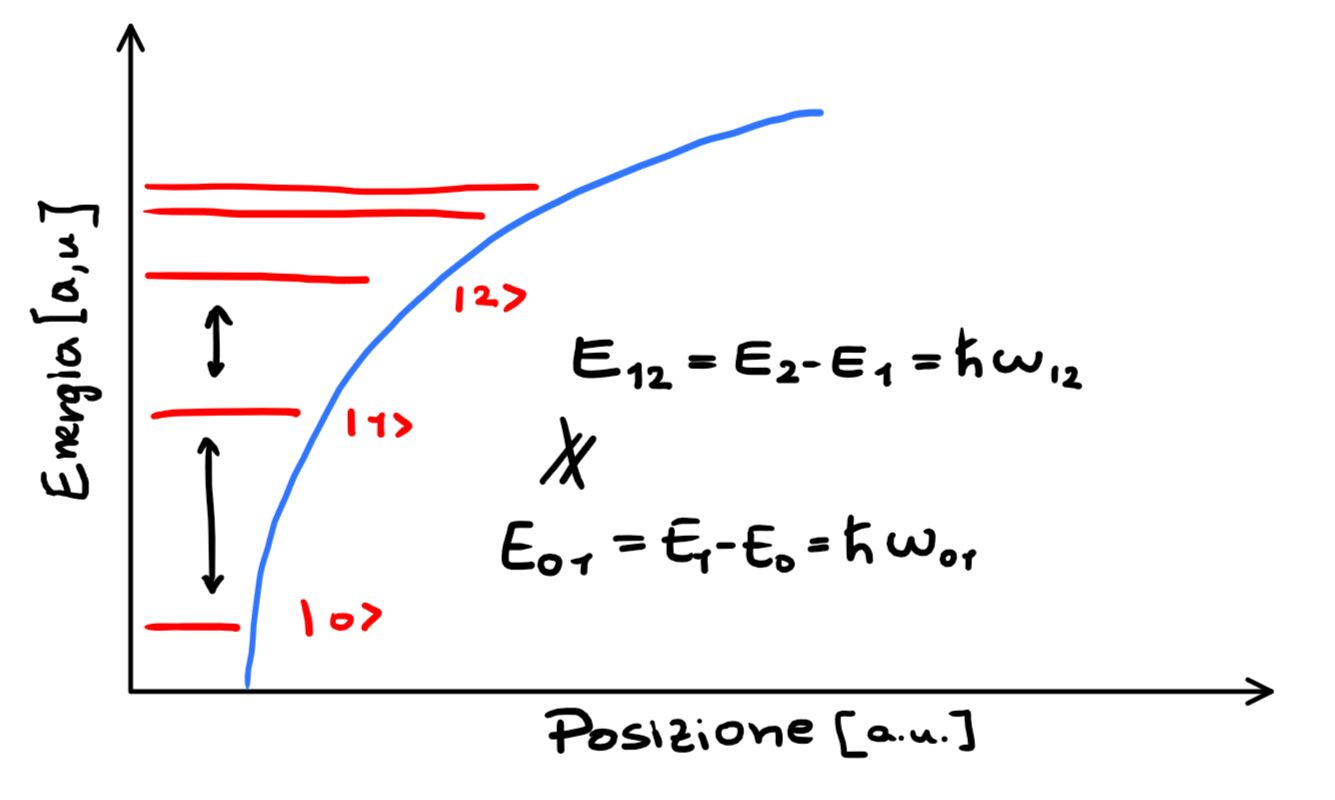
\includegraphics[width=0.6\textwidth]{nature_atom.JPG}
%     \caption{Livelli energetici di un atomo}
%     \label{nature atom}
% \end{figure}
% \FloatBarrier

\begin{wrapfigure}{r}{0.5\textwidth}
  \begin{center}
    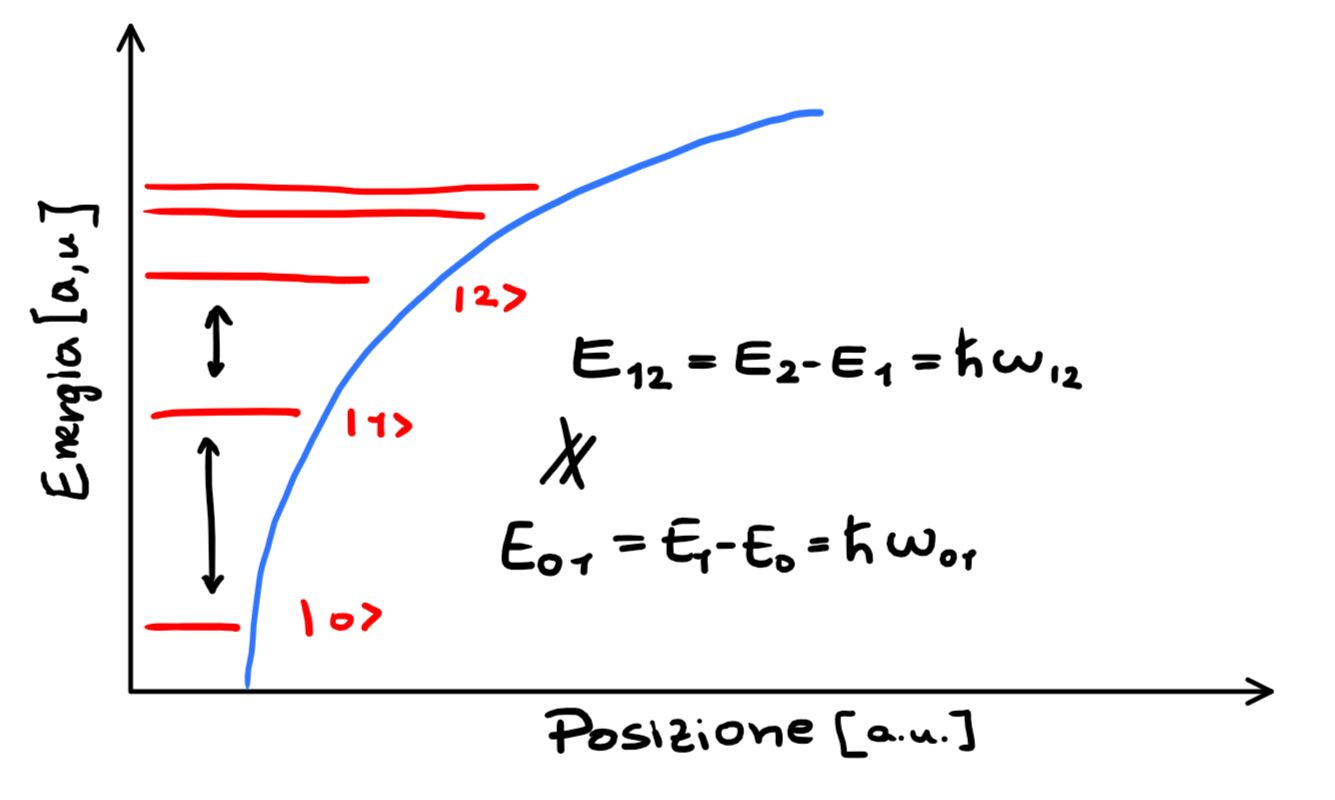
\includegraphics[width=0.48\textwidth]{nature_atom.JPG}
  \end{center}
  \caption{Livelli energetici di un atomo \label{nature atom}}
\end{wrapfigure}


Possiamo selezionare due dei livelli energetici, ad esempio $\ket{0}$ e $\ket{1}$ come i due stati di un qubit.\\
Notiamo che la separazione energetica tra le varie coppie di livelli è diversa (ad esempio $E_{01} \neq E_{12}$).
Questa proprietà è fondamentale. Infatti, se agiamo sull'atomo con un laser alla frequenza $\omega_{01}$, induciamo delle oscillazioni di Rabi tra i livelli $\ket{0}$ e $\ket{1}$, e, dato che $\omega_{01} \neq \omega_{12}$, il sistema rimarrà sempre nel sottospazio generato da  $\ket{0}$ e $\ket{1}$, poiché il laser non ha l'energia opportuna per passare da $\ket{1}$ a $\ket{2}$.\\
Abbiamo dunque un sistema confinato nel sottospazio generato da due stati: \textbf{un atomo è un buon qubit}.\\
Ad esempio, i livelli iperfini del $^9Be^+$ hanno tempi di decadimento\footnote{T$_1$ indica il tempo di decadimento. Ad esempio, se preparo il sistema nello stato $\ket{1}$, T$_1$ indica il tempo che il sistema impiega per decadere nello stato $\ket{0}$ spontaneamente.} e tempi di coerenza\footnote{T$_2$ indica il tempo di coerenza, cioè il tempo per il quale una sovrapposizione di stati rimane coerente.} lunghi:

\begin{center}
    T$_1 \sim$ qualche anno \qquad  \qquad T$_2	\gtrsim$ 10 secondi
\end{center}

\subsection{Atomi artificiali}
Per poter realizzare un qubit, vorremmo ricreare artificialmente un sistema che si comporti come gli atomi presenti in natura.
Costruiamo il più semplice sistema che ci viene in mente, usando un induttanza e una capacità (assumiamo che tutti i componenti del circuito siano superconduttori\footnote{In un superconduttore il passaggio di elettroni avviene senza dissipazione di energia.}).

\begin{figure}[h]
    \centering
    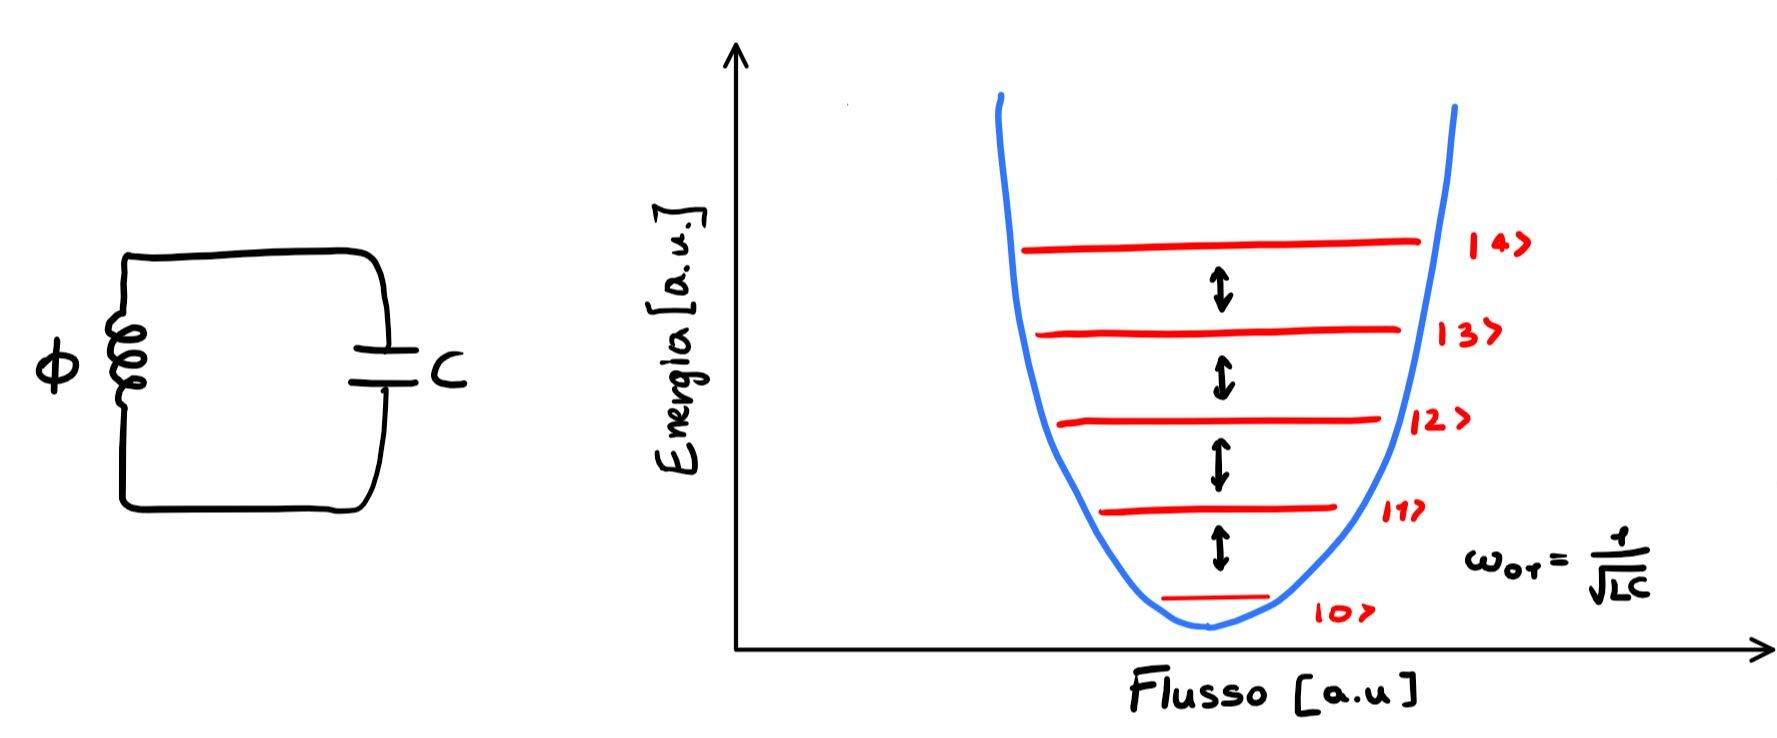
\includegraphics[width=0.65\textwidth]{LC.JPG}
    \caption{Un primo tentativo di modello di qubit: un oscillatore LC.}
    \label{LC}
\end{figure}
\FloatBarrier

Questo sistema ha un'energia caratterizzata da un termine capacitivo e da un termine induttivo:
\begin{equation}
H = \dfrac{Q^2}{2C}+ \dfrac{\Phi^2}{2L}
\label{HLC}
\end{equation}

Dove ricordiamo che il flusso $\Phi$ è dato dall'integrale del potenziale ai capi dell'induttanza: \(\Phi(t) = \int_{-\infty}^{t} V(t') \,dt'\)\\

L'energia in funzione del flusso $\Phi$ è una parabola. Notiamo dunque una corrispondenza con i livelli energetici dell'oscillatore armonico quantistico, che, come sappiamo dalla MQ, sono equispaziati. La separazione energetica, scritta in termini di frequenza, è pari a $\omega_{01} = \frac{1}{\sqrt{LC}}$.\\

%Questo sistema è un buon qubit?\\

Per agire sul sistema, anziché sparargli un laser contro (come nel caso del vero atomo), si usa un generatore di corrente alternata nelle microonde:
\begin{figure}[h]
    \centering
    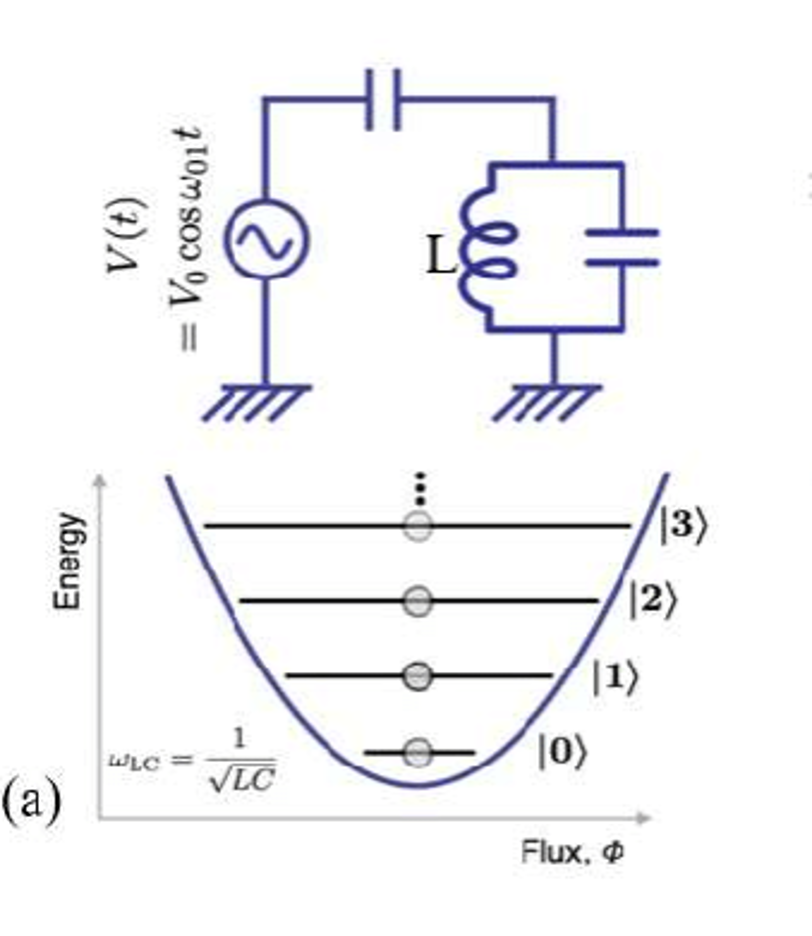
\includegraphics[width=0.37\textwidth]{LC_microwave.png}
    \caption{Oscillatore LC con generatore di corrente alternata nelle microonde.}
    \label{LC_microwave}
\end{figure}
\FloatBarrier

Dato che la separazione energetica è la stessa tra tutti i livelli, una volta che la sorgente di radiofrequenza ha promosso il sistema da $\ket{0}$ ad  $\ket{1}$, non c'è nulla che vieta che il sitema vada da  $\ket{1}$ a  $\ket{2}$ e poi da  $\ket{2}$ a  $\ket{3}$ e così via.
Concludiamo che questo sistema \textbf{non è un buon qubit}.\\

Il punto chiave per ottenere un buon qubit è l'anarmonicità nella separazione energetica tra i livelli: vorremmo ottenere uno spettro non lineare.
Per fare ciò abbiamo bisogno di un elemento non lineare: la \textbf{giunzione Josephson}.

\section{La giunzione Josephson}
La giunzione Josephson (JJ) è sostanzialmente un sandwich tra due pezzi di superconduttori e un isolante.\\
La corrente passa attraverso tale giunzione a causa dell'effetto tunnel delle coppie di cooper\footnote{Una coppia di Cooper è uno stato legato fra due elettroni (oppure anche fra due lacune) che si può realizzare grazie all'intervento di una qualche interazione attrattiva, tale da vincere la forza elettrostatica repulsiva fra le due particelle. I due elettroni legati si comportano non più come fermioni, ma come un bosone. (\url{https://it.wikipedia.org/wiki/Coppia_di_Cooper})}. In particolare vale la seguente relazione tra la corrente $I$ che attraversa la giunzione ed il flusso $\Phi$ ai suoi capi:

\begin{equation}
I = I_0 \sin\left(\dfrac{2\pi\Phi}{\Phi_0}\right)
\label{IJJ}
\end{equation}

\noindent
con:\\
- $I_0$ = corrente critica (parametro della giunzione)\\
- $\Phi_0 = \dfrac{h}{2e}$\\

\noindent
Ricordiamo che per un induttore la relazione tra flusso e corrente è lineare: $I = \frac{\Phi}{L}$. Questa è proprio la definizione di induttanza L.\\

Invece, nel caso della JJ, la relazione tra corrente e flusso \eqref{IJJ} non è lineare. Possiamo comunque definire un'induttanza Josephson (dipendente dal flusso) pari a:
\begin{equation}
    L_J(\Phi) = \left(\dfrac{\partial I}{\partial \Phi}\right)^{-1} = \dfrac{\Phi_0}{2\pi I_0}\dfrac{1}{\cos{(2\pi\Phi/\Phi_0)}}
\end{equation}

In sostanza abbiamo trovato che la giunzione Josephson si comporta in maniera simile ad un'induttanza, nel senzo che lega la corrente al flusso, ma in questo caso tale relazione è non lineare.\\
Dall'equazione \eqref{HLC}, abbiamo che il termine energetico associato all'induttanza va come 1/L. Per cui, nel caso dell'induttanza Josephson $L_J$, abbiamo un termine energetico che va come $\cos{(2\pi\Phi/\Phi_0)}$.

\begin{figure}[h]
    \centering
    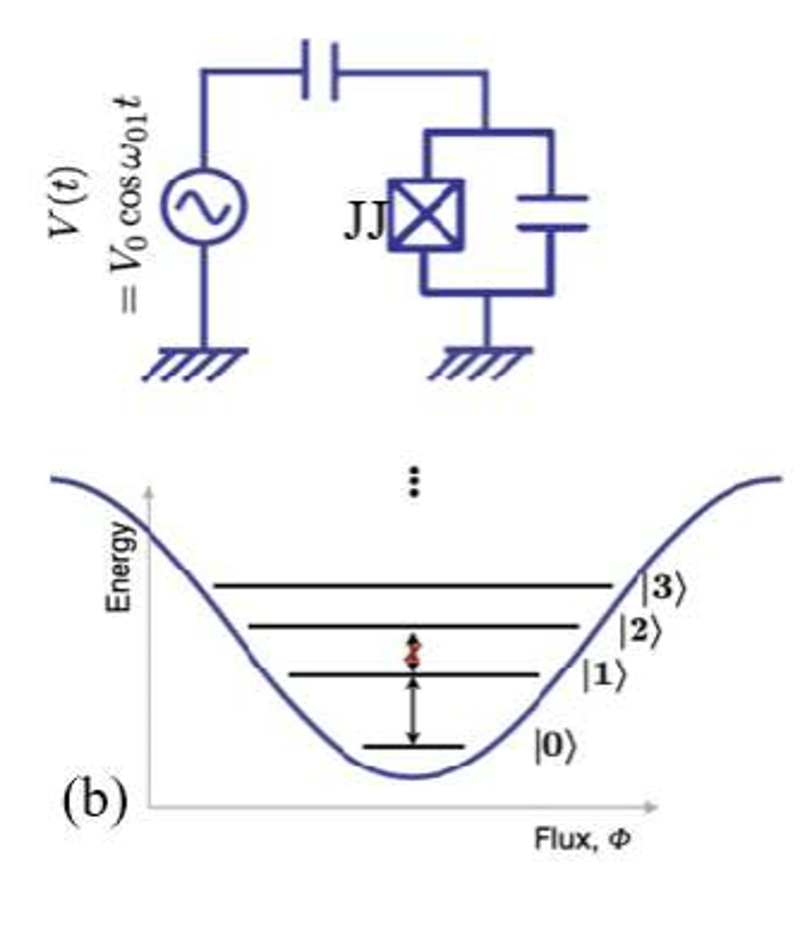
\includegraphics[width=0.37\textwidth]{JJ_energy.png}
    \caption{Come in figura \ref{LC_microwave}, ma sostituiamo all'induttanza una giunzione Josephson.}
    \label{JJ_energy}
\end{figure}
\FloatBarrier

Abbiamo dunque un potenziale anarmonico: i livelli energetici non sono equispaziati, proprio come volevamo. Abbiamo ottenuto un \textbf{atomo artificiale}.\\

\subsection{Hamiltoniana del sistema}
Vogliamo ora studiare il contributo all'hamiltoniana apportato dalla giunzione Josephson.
Sappiamo che l'energia è data dall'integrale temporale della potenza:
\begin{equation}
    E =  \int W(t) \,dt = \int V(t)I(t) \,dt = \int \cancel{dt} \dfrac{d\Phi}{\cancel{dt}} I_0 \sin\left(\dfrac{2\pi\Phi}{\Phi_0}\right) \equiv -E_J\cos\left(\dfrac{2\pi\Phi}{\Phi_0}\right)
\end{equation}

Dove abbiamo definito il parametro $E_J$, noto come Energia Josephson\footnote{Le coppie di cooper tunnellano avanti-indietro attraverso la giunzione. $E_J$ è legato alla frequenza con cui avvengono tali oscillazioni di coppie di cooper.}.\\



Dunque, se vogliamo operare il sistema tra gli stati $\ket{0}$ e $\ket{1}$, dobbiamo applicare una tensione alternata alla frequenza $\omega_{01}$.
Possiamo anche sostituire il generatore di tensione alternata con un generatore DC:

\begin{figure}[h]
    \centering
    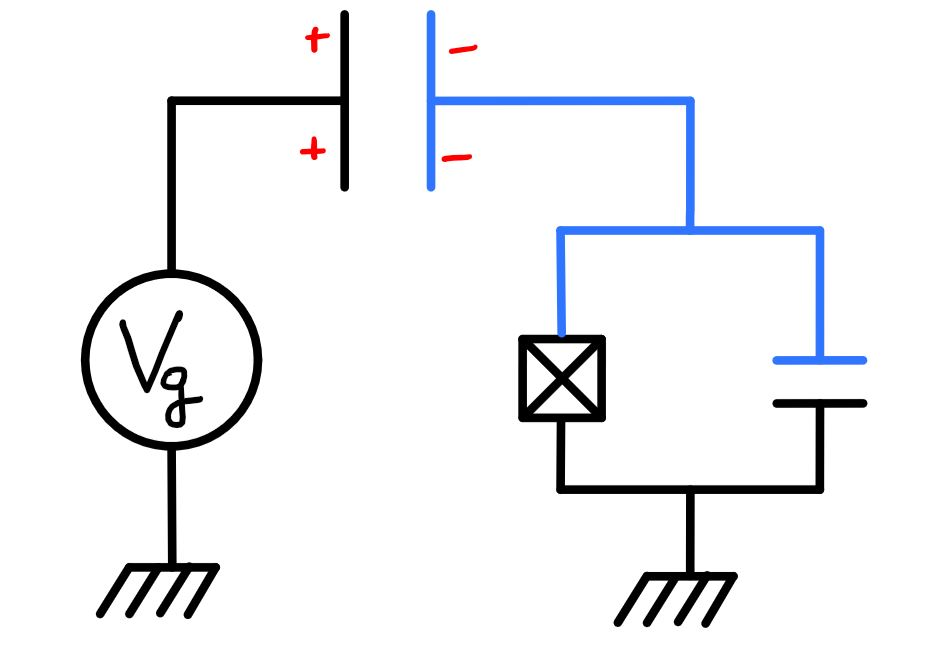
\includegraphics[width=0.35\textwidth]{DC_island.JPG}
    \caption{Sostituiamo il generatore di tensione alternata con un generatore in DC}
    \label{dc}
\end{figure}
\FloatBarrier

In questo caso, il condensatore si caricherà, creando una separazione di cariche. In particolare, la carica totale presente sull'\textit{isola} in blu, sarà la carica dovuta alla JJ più la carica dovuta al condensatore caricato da $V_g$.
Per cui la carica totale presente sull'isola è data da $e$ per due volte il numero di coppie di cooper che attraversano la JJ verso l'isola blu, più l'equivalente applicato dall'esterno ($n_g$).\\
\textbf{Nota:} $n_g$ è una variabile continua che si può settare dall'esterno variando $V_g$.\\


Dunque alla fine otteniamo l'Hamiltoniana completa (passando anche alla notazione con gli operatori):




%$$\hat{H}=\dfrac{\hat{Q}^2}{2C}-E_J\cos\left(\dfrac{2\pi\hat{\Phi}}{\Phi_0}\right)$$


\begin{align} 
\hat{H} &= 
\dfrac{\hat{Q}^2}{2C}-E_J\cos\left(\dfrac{2\pi\hat{\Phi}}{\Phi_0}\right) = \notag\\ 
&= \dfrac{(2e)^2}{2C}\hat{n}^2 - E_J\cos\hat{\varphi}= \notag\\
&=4E_C(\hat{n}-n_g)^2 - E_J\cos\hat{\varphi}
\label{Hfin}
\end{align}

Dove abbiamo usato:
$$ \hat{\varphi} \equiv \dfrac{2\pi\hat{\Phi}}{\Phi_0} $$

%$$ \Phi_0 \equiv \dfrac{h}{2e} $$

$$ \hat{Q} = 2e\hat{n} $$
$$ E_c = \dfrac{e^2}{2C}$$

%$$\hat{H}=4E_C(\hat{n}-n_g)^2 - E_J\cos\hat{\varphi}$$

$E_C$ è l'energia per portare una carica dall'$\infty$ e metterla sulla capacità (Charging Energy).\\

Nella realtà ci sarà del rumore proveniente dall'environment, che cambierà localmente la carica presente sull'isola in blu. Possiamo rappresentare tale rumore come una batteria che varia in maniera casuale la tensione ai suoi capi:

\begin{figure}[h]
    \centering
    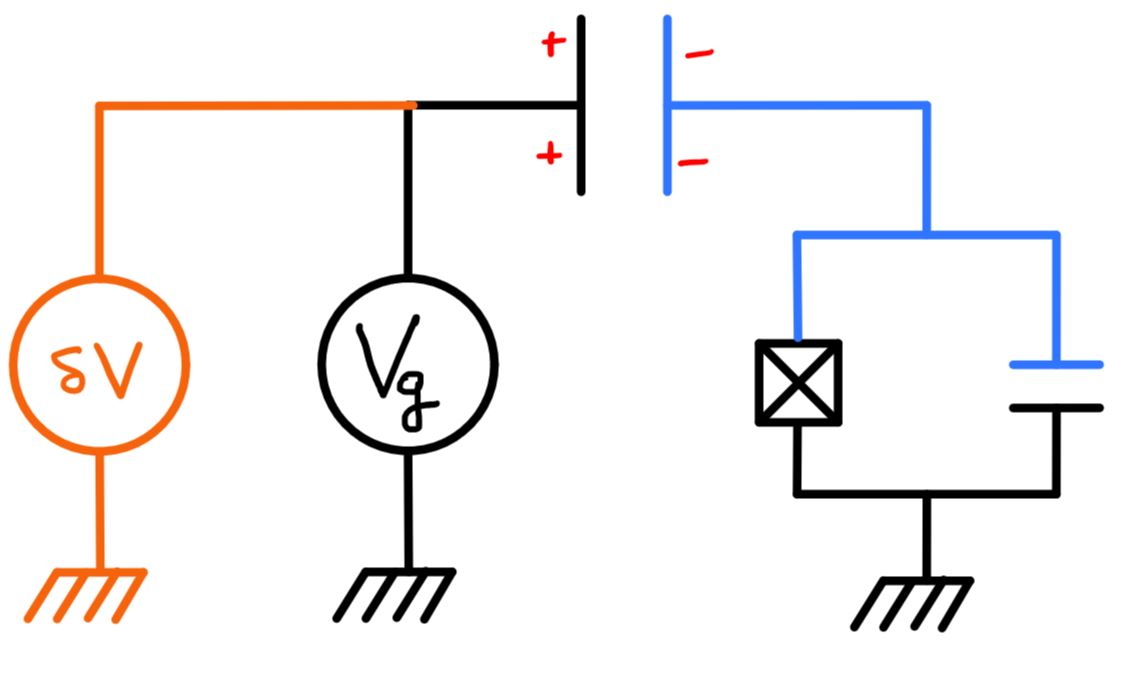
\includegraphics[width=0.4\textwidth]{DC_noise.JPG}
    \caption{Schematizzazione del rumore ambientale.}
    \label{dcnoise}
\end{figure}
\FloatBarrier


Vogliamo capire qual è la scelta ottimale dei parametri $E_J$ ed $E_c$ (quindi del rapporto $E_J/E_C$) in modo da minimizzare l'effetto del rumore.
Studiamo l'effetto che questi parametri hanno sugli autostati dell'energia.

\begin{figure}[h]
    \centering
    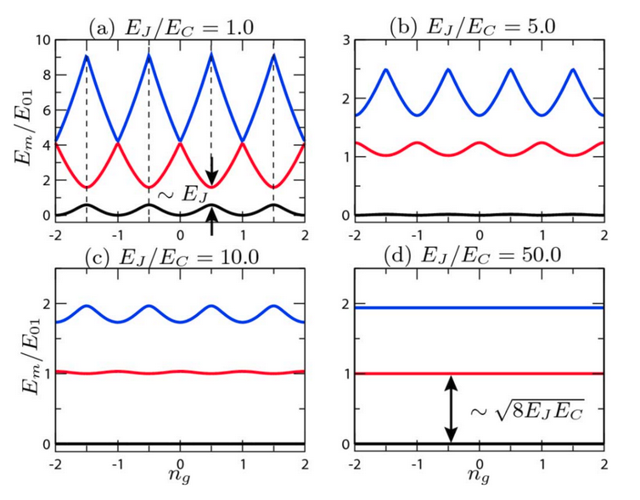
\includegraphics[width=0.6\textwidth]{EJEC.png}
    \caption{Energie dei primi tre livelli energetici (m=0, 1, 2) dell'hamiltoniana \eqref{Hfin}, in funzione della carica di offset $n_g$, per diversi valori del rapporto $E_J/E_C$.}
    \label{ejec}
\end{figure}
\FloatBarrier


\begin{wrapfigure}{r}{0.4\textwidth}
  \begin{center}
        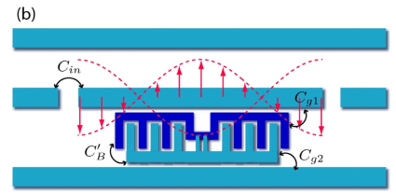
\includegraphics[width=0.35\textwidth]{trasmon2.png}
  \end{center}
  \caption{Struttura a pettine della capacità. \label{pettine}}
\end{wrapfigure}


(a) Scelgo $n_g$ appositamente in modo che piccole variazioni di tale valore, risultino in piccole variazioni nelle energie dei livelli (sweet spot).\\ 
Tuttavia vorremmo migliorare ancora di più la cosa, facendo in modo che qualunque variazione di $n_g$ dovuta al rumore, non porti ad una variazione significativa delle energie.\\
Per farlo si sceglie $E_J \gg E_C$ (d). In pratica questo si ottiene aumentando il valore della capacità,  e quindi diminuendo $E_C$.

Per aumentare la capacità, di solito si utilizza una struttura a pettine, che aumenta la superficie delle due armature, come si vede in figura \ref{pettine}.

% \begin{figure}[h]
%     \centering
%     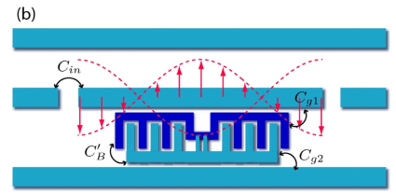
\includegraphics[width=0.4\textwidth]{trasmon2.png}
%     \caption{Capacità.}
%     \label{C}
% \end{figure}
% \FloatBarrier



Nelle condizioni della sottofigura (d), abbiamo che per qualunque valore di $n_g$ il qubit opererà in maniera ottimale. Questo è quello che si chiama (Transmon Regime).\\

Una quantità utile per stimare l'efficienza del nostro qubit è la dispersione, che indica di quanto varia al massimo l'escursione di energia di un livello energetico, al variare di $n_g$.

\begin{figure}[h]
    \centering
    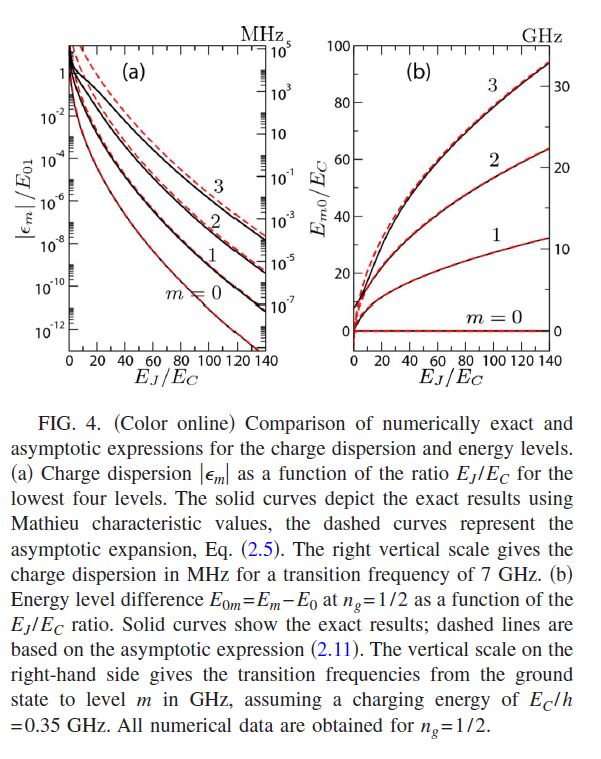
\includegraphics[width=0.63\textwidth]{dispersion.JPG}
    \caption{}
    \label{disp}
\end{figure}
\FloatBarrier

Osserviamo che la dispersione decade esponenzialmente all'aumentare del rapporto $E_J/E_C$. Nello specifico $\propto e^{-\sqrt{8E_J/E_C}}$. Questo ci piace.\\
Tuttavia se osserviamo la spaziatura tra i livelli nel caso (d), questi sembrano essere equispaziati, e questo non ci piace per un qubit. Un indice di quanto i livello sono equispaziati è rappresentato dall'anarmonicità relativa, che possiamo plottare in funzione di $E_J/E_C$.
L'armonicità relativa è definita come $$\alpha \equiv E_{12}-E_{01}, \qquad \quad \alpha_r=\alpha/E_{01}$$


\begin{figure}[h]
    \centering
    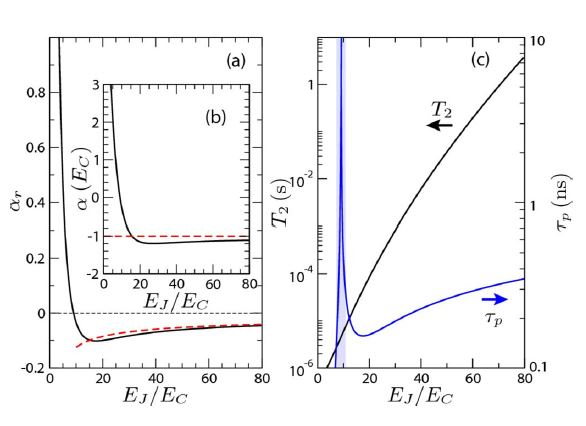
\includegraphics[width=0.55\textwidth]{anarmonicity.JPG}
    \caption{Anarmonicità relativa (a) e assoluta (b)}
    \label{an}
\end{figure}
\FloatBarrier

\begin{equation}
    \alpha \approx -E_C \qquad \quad \alpha_r \approx -(8E_J/E_C)^{-1/2}
    \label{anharmonicity}
\end{equation}


\textit{Employing \eqref{anharmonicity}, we find that the energy ratio should
satisfy $20 \lesssim  E_J/E_C \ll 5 \times 10^4$, opening up a large range with exponentially decreased sensitivity to charge noise and yet sufficiently large anharmonicity for qubit operations. In other words, the transmon regime is reached without paying any serious penalty, and pulse generation techniques common for CPB qubits can directly be transferred to the transmon qubit.}

\section{Impiego dei transmoni per la rivelazione dei singoli fotoni nelle microonde.}


Vogliamo ora capire come i transmoni possano essere sfruttati per la rivelazione di particelle assioniche.\\
In presenza di un campo magnetico statico, il campo assionico e il campo elettromagnetico interagiscono in modo tale che un assione possa convertire in un fotone la cui energia è circa pari alla massa a riposo dell’assione. In termini di frequenza, il range favorevole per i fotoni così prodotti è 500MHz-500GHz.\\

 Dunque si costruiscono delle cavità risonanti (\textit{microwave cavities}) con frequenza di risonanza opportuna, che possano accumulare i fotoni prodotti nelle rare occasioni in cui avviene la riconversione assione-fotone descritta in precedenza. Nelle condizioni sperimentali tipiche, si stima un numero medio di fotoni per misurazione, pari a $\Bar{n}_{axion}\sim 10^{-8}-10^{-5}$.

Attualmente, questi esperimenti utilizzano amplificatori lineari che operano al limite dello SQL (Standard Quantum Limit), le cui fluttuazioni corrispondono ad un background effettivo pari a $\Bar{n}_{SQL}=1$. Dunque è chiaro che il rumore quantistico copre completamente il segnale, rendendo impossibile la rivelazione ($\Bar{n}_{SQL}\gg\Bar{n}_{axion} $).\\

Esistono già delle tecnologie che funzionano bene per rivelare singoli fotoni nell’infrarosso, ma non vanno altrettanto bene quando si tratta di fotoni di bassa energia nelle microonde.\\
E’ qui che entrano in gioco i transmoni. Per rivelare i singoli fotoni, si sfrutta l’interazione tra un qubit superconduttore e il campo elettromagnetico nella cavità risonante.\\
In particolare, usando questa tecnica, si può sviluppare una misura QND (Quantum nondemolition) che possa essere ripetuta più volte in modo da migliorare l’efficienza nel conteggio dei fotoni e sopprimere i “dark-count”.

\begin{figure}[h]
    \centering
    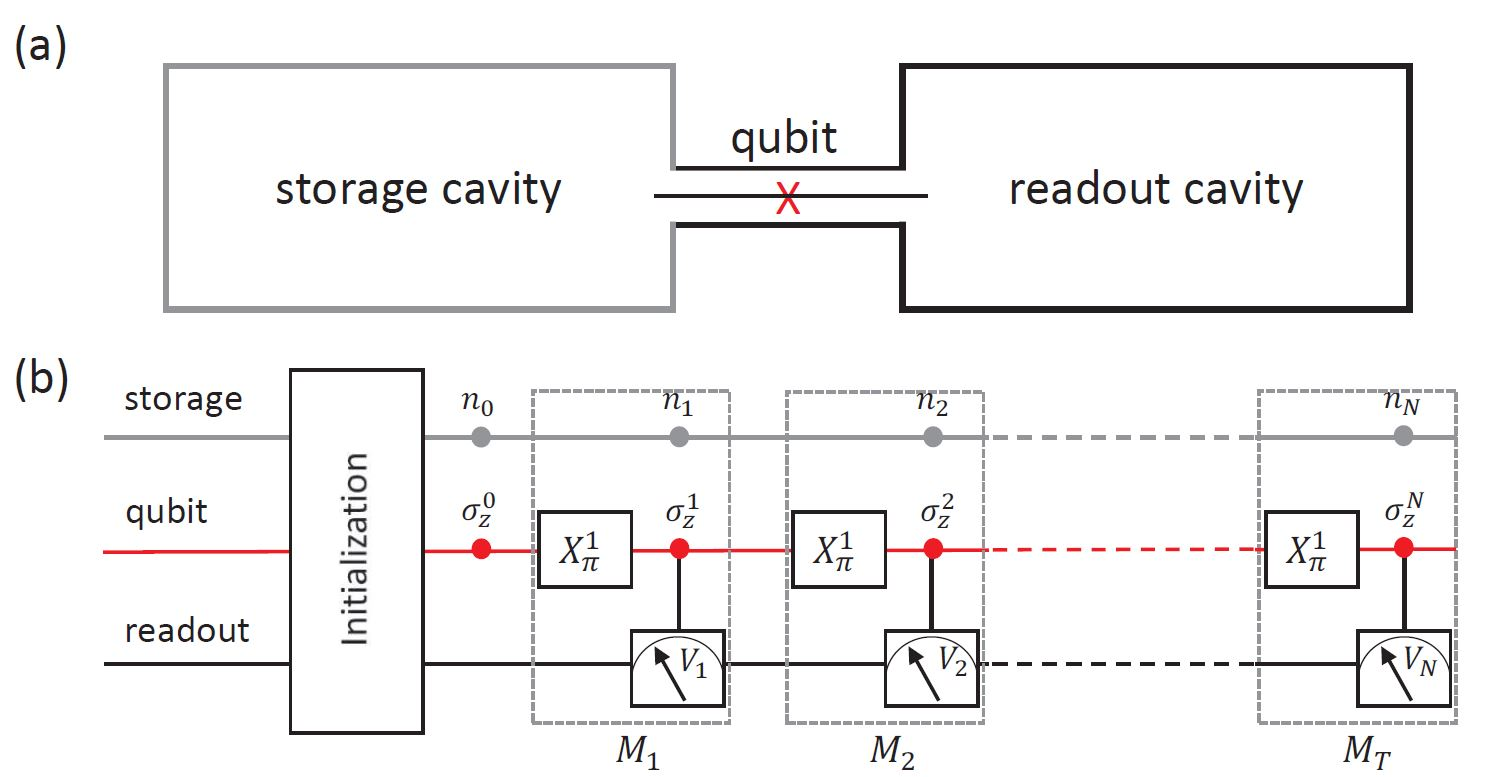
\includegraphics[width=0.63\textwidth]{cavity.JPG}
    \caption{(a) Apparato sperimentale per la misura del numero di fotoni.\\ (b) Protocollo di misura.}
    \label{app}
\end{figure}
\FloatBarrier

L’apparato sperimentale è costituito da un trasmone accoppiato a due cavità: una di accumulazione e una di lettura. In presenza di un forte campo magnetico statico, la cavità di accumulazione è usata per accumulare fotoni risonanti convertiti da assioni, ed ha un alto quality factor per lo storage di fotoni.\\
Invece la cavità di lettura è una cavità superconduttrice standard, con un basso quality factor per una lettura più veloce dello stato del qubit.\\

La presenza di un fotone nella cavità comporta uno shift nella frequenza di transizione del qubit. In particolare, ogni fotone comporta uno shift nella frequenza pari a 2$\chi$ .

\begin{figure}[h]
    \centering
    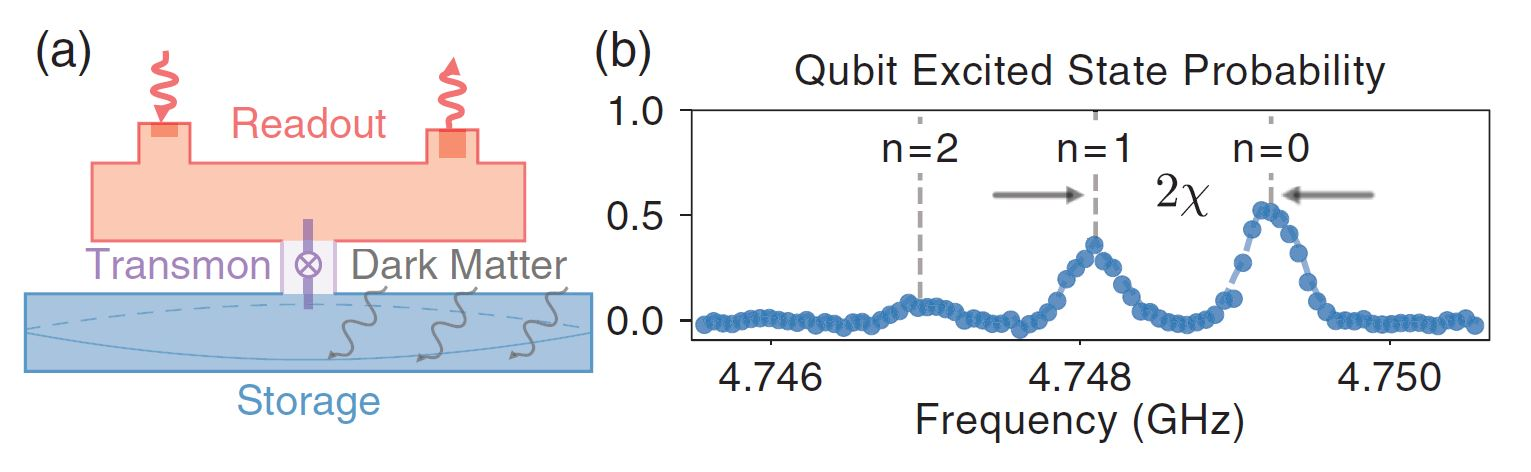
\includegraphics[width=0.63\textwidth]{qubit_freq.JPG}
    \caption{Frequenza di risonanza del qubit al variare del numero di fotoni nella cavità.}
    \label{shift}
\end{figure}
\FloatBarrier

\subsection{Protocollo di misurazione}
Il protocollo di misurazione procede come segue:\\
\begin{itemize}
    \item Per prima cosa si applica un impulso $\pi$ ($X^1_\pi$) al qubit: questo ha l’effetto di flippare lo stato del qubit se e solo se c’è esattamente un fotone nella cavità.
    \item Successivamente, lo stato del qubit $\sigma_z$ è misurato sfruttando l’accoppiamento della cavità di lettura con il qubit.
\end{itemize}

Questi due passaggi permettono di sondare il numero di fotoni nella cavità di accumulazione. Ripetendo questa procedura è possibile monitorare la comparsa/scomparsa di fotoni nella cavità. Nello specifico, questa procedura è sostanzialmente “quantum non-demolition\footnote{il concetto di misure ”quantum
non-demolition” (abbreviato QND), che indica un insieme di misure quantistiche in cui l’osservabile
misurata viene disturbata il meno possibile: pi`u precisamente, si cerca di fare in modo che l’indeter-
minazione di tale misura non aumenti a causa della misura stessa, in modo che misure ripetute diano
lo stesso risultato, o pi`u in generale che tale risultato sia predicibile. Come vedremo pi`u avanti, que-
sto permette di superare i cosiddetti standard quantum limit (SQL), ovvero dei limiti alla precisione
della misura dovuti a effetti di natura quantistica, in particolare al principio di indeterminazione di
Heisenberg}”.\\

Facciamo N misure. Studiamo ogni misura in correlazione con quella precedente: se lo stato del qubit non flippa, vuol dire che nella cavità non è presente alcun fotone. Se lo stato flippa, allora c’è un fotone nella cavità. Questo idealmente.\\

Nella realtà ci sono diverse imperfezioni di cui tenere conto: Errori nella lettura del qubit; Decadimenti $T_1$ che consistono nel qubit che passa spontaneamente dal gs allo stato eccitato o viceversa.\\

Nella seguente figura c’è un esempio di una serie di misure sullo stato del qubit, in cui si vede l’effetto delle imperfezioni sul numero di fotoni ottenuto semplicemente correlando ogni misura con la successiva.


\begin{figure}[h]
    \centering
    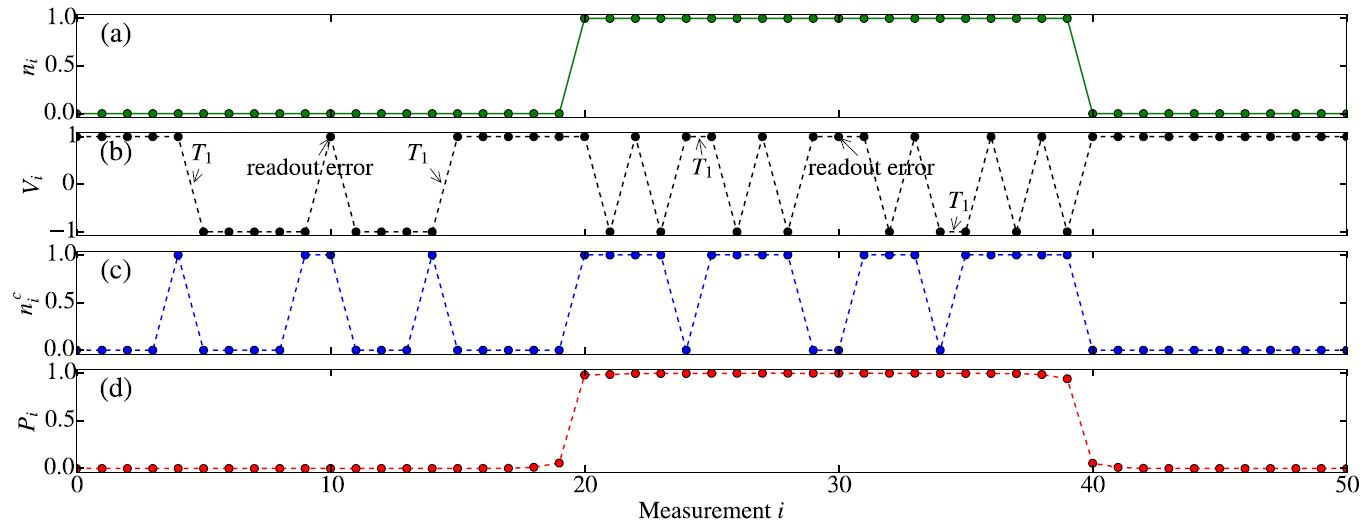
\includegraphics[width=1\textwidth]{measures.JPG}
    \caption{An Example of (a) photon state $n_i$ and (b) the readout voltage $V_i$ after digitizing qubit $\ket{g}$ to +1 and $\ket{e}$ to -1. $T_1$ jumps and readout errors are pointed out by the arrows. (c) Photon number $n_i^c$ inferred from correlating the neighboring readout voltages $V_i$ and $V_{i+1}$. (d) Probability $P_i = P(n_i = 1|V_1\cdots V_N)$ that one photon is present in the cavity of the time of the $i^{th}$ measurement obtained from applying the Bayesian smoothing algorithm to the entire measurement record. The lines are a guide to eye.}
    \label{meas}
\end{figure}
\FloatBarrier

La figura \ref{meas} mostra un esempio di una serie di misure effettuate sul qubit, ed evidenzia l'effetto di imperfezioni sul numero di fotoni dedotto usando solamente la correlazione tra misure vicine.\\

Ogni salto $T_1$ (up or down) introduce un errore nella misura del numero di fotoni.\\
Si sceglie una soglia per digitalizzare il \textit{readout voltage} V in +1 per $\ket{g}$ e in -1 per $\ket{e}$. Un'errore di readout comporta un'interpretazione errata dello stato del qubit (\textit{g} anziché \textit{e} o viceversa), e produce due errori consecutivi sul numero di fotoni dedotto, come mostrato in figura \ref{meas}(c).\\

\textit{From Fig. \ref{meas}(c), it
is clear that the experimental imperfections can greatly
hinder our ability to distinguish zero-photon and one-photon
states if we rely solely on correlating neighboring
qubit readouts.}\\

\'E possibile sviluppare un algoritmo di smoothing Bayesiano, che tiene conto dell'intero record di misure per stimare al meglio il numero di fotoni in ogni interrogazione.\\

\textit{Fig. \ref{meas}(d) shows the conditional probability of the
one-photon state obtained from applying the smoothing algorithm to the example data in Fig. \ref{meas}(b). Compared
to Fig. \ref{meas}(c), it is clear that the errors introduced by $T_1$
jumps and readout errors are very effectively corrected
after filtering based on the entire measurement record.}

\end{document}